\chapter{Experimentelle Ergebnisse}
\label{chap:results}
	In diesem Kapitel wird detailliert geschildert, auf welche Weise die Experimente mit der Differentiellen Evolution durchgeführt worden sind. Im Anschluss werden die daraus erzielten Ergebnisse präsentiert und interpretiert.
	
	\section{Testbedingungen}
	\label{sec:execution}
	
		\subsection{Auswahl an Bildmaterial}
		\label{sub:choice-of-images}
			Zur Evaluierung der Differenziellen Evolution werden insgesamt 30 Bilder herangezogen. Davon weisen 15 Bilder einen laser gravierten Zeichencode wie in Abbildung \ref{fig:example-code}a auf, während die restlichen 15 Bilder einen gestempelten Code nach dem Muster aus \ref{fig:example-code}b vorweisen. Jedes Bild wird dabei zweimal ausgewertet: einmal mit und einmal ohne Mittelwertfilter.\\
			Der Unterschied zwischen den jeweiligen Bildern ist in Abbildung \ref{fig:filter} wiedergegeben:
			\begin{figure}[H]
				\centering
				\subfloat[][Bauteil mit gelasertem Code ohne Mittelwertfilter]{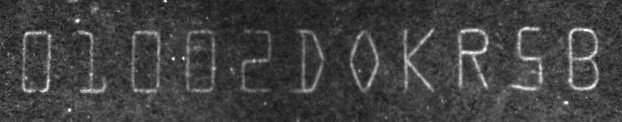
\includegraphics[width=0.48\linewidth]{IMG_01002DOKR5B_c}}
				\quad
				\subfloat[][Bauteil mit gelasertem Code mit Mittelwertfilter]{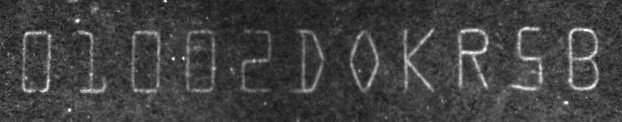
\includegraphics[width=0.48\linewidth]{IMG_01002DOKR5B_c}}
				
				\subfloat[][Bauteil mit gestempeltem Code ohne Mittelwertfilter]{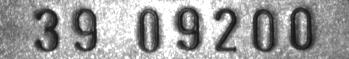
\includegraphics[width=0.48\linewidth]{IMG_3909200}}
				\quad
				\subfloat[][Bauteil mit gestempeltem Code mit Mittelwertfilter]{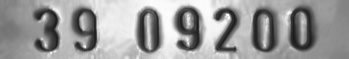
\includegraphics[width=0.48\linewidth]{IMG_3909200-denoised}}
				\caption{Unterschied zwischen Bildern ohne und Bildern mit Mittelwertfilter}
				\label{fig:filter}
			\end{figure}
	
		\subsection{Parameter-Wahl}
		\label{sub:de-params}
			Die einstellbaren Parameter für den implementierten Algorithmus der Differenziellen Evolution und die nachfolgende Segmentierung setzen sich wie folgt zusammen:\\
			Die für den Algorithmus relevanten Parameter belaufen sich auf den Mutationsfaktor $F$, den Crossover-Faktor $C_{r}$ und die maximale Anzahl an Iterationen $G$. Im vorliegenden Test-Szenario wurden $F = 0.5$ und $C_{r} = 0.9$ gewählt. Den Parameter $G$ betreffend wurde eine Unterscheidung getroffen zwischen den Segmentierungsmodellen in den Abschnitten \ref{sec:meth1} und \ref{sec:meth2} respektive. Dementsprechend wurden mit dem Modell der Gaußschen Approximation vier Durchläufe mit $G \in \{100, 200, 500, 1000\}$ ausgeführt, wohingegen anhand des K-Means-Clustering-Modells wegen des deutlich erhöhten Rechenaufwandes im Vergleich mit der Gaußschen Approximation lediglich vier Ausführungssequenzen mit $G \in \{5, 10, 20, 50\}$ absolviert wurden.\\
			In dieser Konstellation werden die Tests für eine Segmentierung in $K$ Klassen mit $K \in \{2,3,4,5\}$ durchgeführt.

	\section{Implementierung der Test-Applikation}
	\label{sec:implementation}
		\subsection{Workflow}
		\label{sub:workflow}
			\begin{figure}[H]
				\centering
				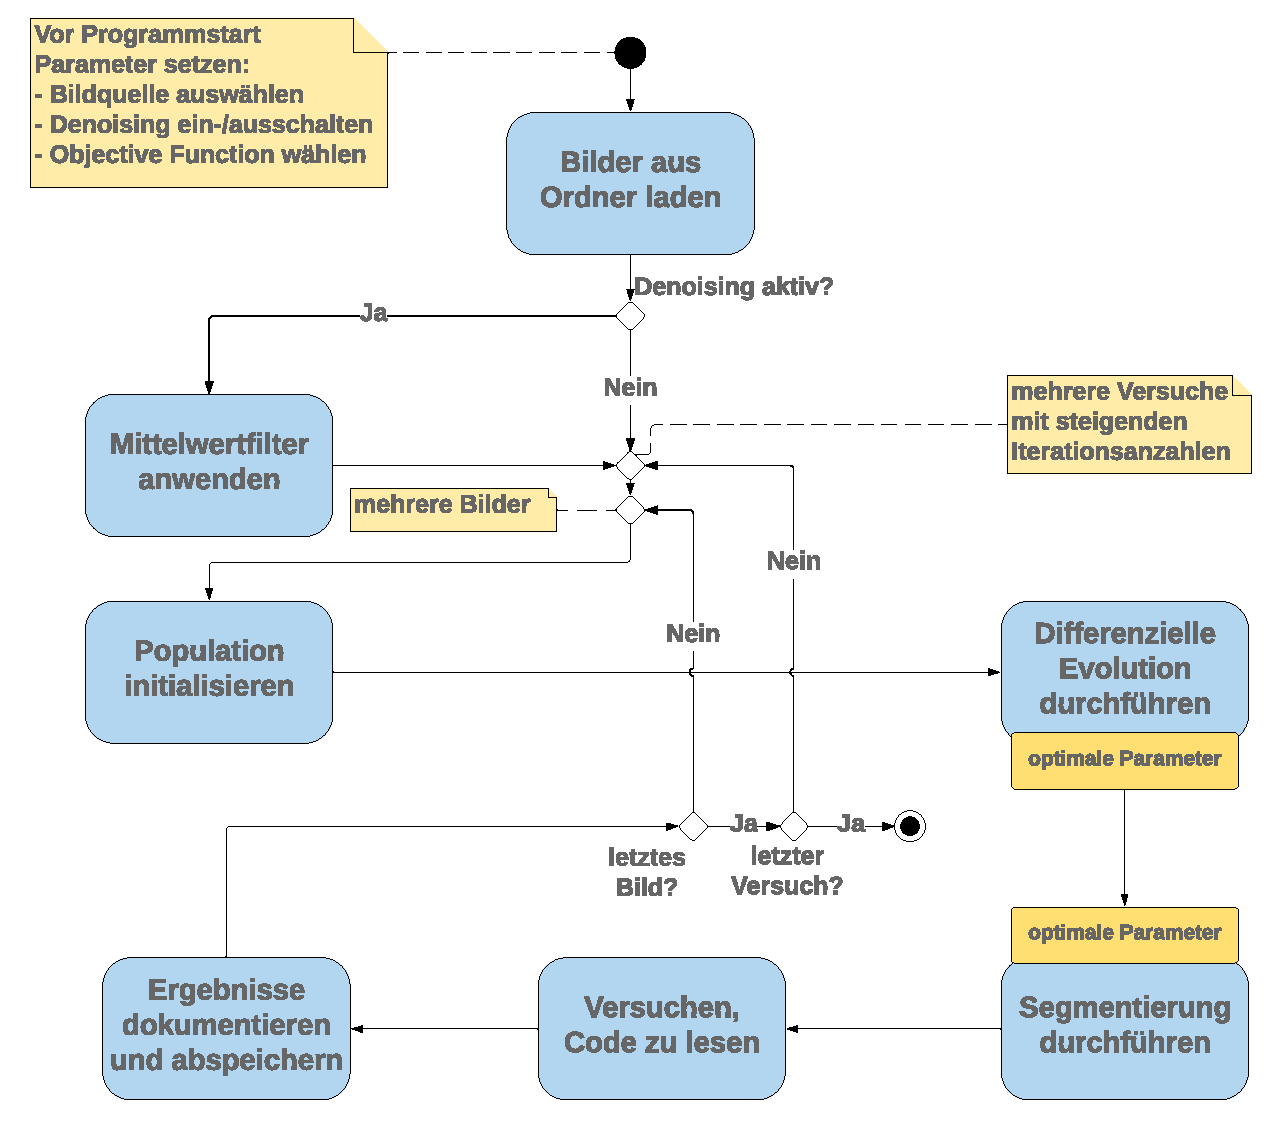
\includegraphics[width=\linewidth]{diff-evol-activity}
				\caption{Aktivitätsdiagramm des Ablaufs in der Test-Applikation}
				\label{fig:diff-evol-activity}
			\end{figure}
			Aus Abbildung \ref{fig:diff-evol-activity} lassen sich die Abläufe entnehmen, die im während dieser Arbeit entwickelten Test-Programm abgehandelt werden:\\
			Vor dem Programmstart muss die Wahl der Bildquelle und des Segmentierungsmodells (künftig als \textit{Objective Function} bezeichnet) getroffen werden. Zusätzlich wird festgelegt, ob ein Mittelwertfilter angewendet werden soll. \\
			Bei Programmstart werden sodann die entsprechenden Bilder geladen und gegebenenfalls mit dem Mittelwertfilter vorbehandelt. Nach diesen Vorbereitungen wird für jedes geladene Bild die Population initialisiert und dem \gls{de}-Algorithmus übergeben. Dieser wird wiederum sukzessiv für jedes $G$, wie in Paragraph \ref{sub:de-params} beschrieben, aufgerufen. Mit dem Ergebnis aus jedem Durchlauf wird dann eine Segmentierung des Bildes anhand der zuvor gewählten \textit{Objective Function} durchgeführt und es folgt ein Versuch, den Code zu lesen. Das jeweilige Resultat hieraus wird schließlich in einer \textit{CSV-Datei} dokumentiert.
	
		\subsection{Wahl der Programmiersprache}
		\label{sub:prog-lang}
			Auf dem Gebiet der Bildverarbeitung haben sich im Allgemeinen zwei Programmiersprachen bewährt - \textit{Python} und \textit{C++} - nicht zuletzt wegen der in der Praxis oft verwendeten Open-Source-Bibliothek \textit{OpenCV}, die für diese beiden Sprachen eine Anwendungsschnittstelle bereitstellt (siehe Online-Dokumentation). Für diese Arbeit ist die Wahl auf die Sprache Python gefallen, da sie gegenüber C++ einige Vorteile mit sich bringt \cite[S. 21f]{python-book}:\\
			Es bietet erhöhte Lesbarkeit sowie Benutzbarkeit aufgrund der Loslösung von der darunterliegenden physischen Schicht. Oft beträgt der Umfang eines Python-Skripts lediglich bis zu einem Drittel der Größe eines äquivalenten C++-Programms. Somit lassen sich mit Python auch komplexere Applikationen in einem kürzeren Zeitrahmen erstellen als mit C++. 

		\subsection{Benutzte Module}
		\label{sub:used-modules}
			Nachstehend ist eine Auflistung jener hier verwendeten Python-Module, die essenziell für die Anfertigung dieser Arbeit waren, zum Zwecke der Nachvollziehbarkeit zu finden:\\
			Für diverse Plots, wie sie in Abschnitt \ref{sec:results} zu finden sind, wurde das \textit{mathplotlib}-Modul in der Version $3.1.0$ eingesetzt. Für die dieser Arbeit zugrundeliegende Aufgabe war unter anderem das \textit{numpy}-Package, das hier unter der Version $1.16.4$ Anwendung findet, unabdingbar. Es bietet eine umfangreiche array-ähnliche Datenstruktur an, womit sich vor allem Matrix-Operationen mit geringem Aufwand realisieren lassen. Zudem 
		
	\section{Ergebnisse}
	\label{sec:results}
	
		\subsection{Vergleich Modell 1 - Modell 2}
		\label{sub:comp-m1-m2}
		
		\subsection{Vergleich unterschiedlicher Bildgruppen}
		\label{sub:comp-diff-images}
		
		\subsection{Einfluss von Denoising auf das Ergebnis}
		\label{sub:influence-of-denoising}
		
		\subsection{Beurteilung des Ergebnisses bei steigender Iterationszahl}
		\label{sub:judging-higher-iteration}